\documentclass[english,12pt]{article}
\usepackage[]{geometry}
\usepackage{tabularx}
\usepackage{blindtext}
\usepackage{enumerate}
\usepackage{parskip} 
\usepackage{siunitx}
\usepackage{amsmath}
\usepackage{amsfonts}
\usepackage{amssymb}
\usepackage{hyperref}
\usepackage{listings}
\usepackage{inconsolata}
\usepackage{parskip}
\usepackage{graphicx}
\usepackage{wrapfig}
\usepackage{float}
\usepackage{titlesec}
\usepackage{blindtext}
\usepackage{longtable}
\usepackage{multicol}
\usepackage{varwidth}
\usepackage{multirow}
\usepackage{booktabs}
\usepackage{fancyhdr}
\usepackage[svgnames,table]{xcolor}
\usepackage[tableposition=above]{caption}
\usepackage{pifont}
\usepackage{array,ragged2e}
\newcolumntype{P}[1]{>{\RaggedRight\arraybackslash}p{#1}}
% Styling
\titleformat{\section}{\large\bfseries}{\thesection}{1em}{}
\addtolength{\topmargin}{-2.5pt}
\fancyhead{}
\pagestyle{fancy}
\fancyhead[L]{CSE/IT 326 - Software Engineering}
\fancyhead[R]{2/13/25}
\hfuzz=0.64pt % Allow hbox to overflow slightly

\begin{document}

\begin{titlepage}
    \null
    \vspace*{2cm}
    
    \begin{center}
        {\Huge \bfseries CSE 326: Software Engineering}\\[1.5cm]
        {\Large \bfseries Final Project Proposal \& Plan}\\[2cm]
        
        \textbf{Authors:} \\[0.5cm]
        Cole Johnson - \textit{cole.johnson@student.nmt.edu}\\
        Colin Grandjean - \textit{colin.grandjean@student.nmt.edu}\\
        John Runyon - \textit{john.runyon@student.nmt.edu}\\
        Lauren Giles - \textit{lauren.giles@student.nmt.edu}\\[1cm]
        
        New Mexico Institute of Mining and Technology\\
        Socorro, NM 87801, USA\\[2cm]
        
        {\large Date: February 13, 2025}
    \end{center}
    
    \vfill
    \hrule
    \smallskip
    \centerline{\sc New Mexico Tech}
    \smallskip
    \hrule
\end{titlepage}

{\tableofcontents} 
\pagebreak
\section{Introduction}

\subsection{Project Overview and Statement of Proposal}
OCR (Optical Character Recognition) is a technique that a program can use to 
parse individual or stream images into a matched set of some written alphabet; 
often just a set of alphanumeric characters. 
OCR is used in banking, note taking applications,
 and many other services used on a daily basis. 
One of the most common implementations of OCR is the use of neural networks, 
often through supervised learning methods. 
We propose to create a simple neural network that will be trained and tested 
to classify a single image into an alphanumeric character 
using one such supervised learning technique. 
In the process of developing the neural network, 
we'll develop a host of tools to test and 
view the networks created and some performance metrics to gauge effectiveness.

\subsection{Project Scope and Objectives}
The initial scope of the project, as outlined in the overview, will be to create a simple Optical Character Recognition (OCR) system using a neural network and employ supervised learning techniques to test and train our model. Our main objectives for the project include:
\begin{enumerate}[(a.)]
  \item Build the components of neural network using object-oriented design principles and programming language (like Java).
  \item A training and test environment for our neural network.
  \item A graphical user interface (GUI) that the user can draw characters
    for the model to classify them.
  \item A graphical user interface (GUI) to view the created neural networks to
    visually see how each model works.
\end{enumerate}

\section{Risk Management Strategy}

\subsection{Risk Table}
\begin{varwidth}[t]{.5\textwidth}
  \textbf{Category Values}
  \begin{itemize}
    \item \textbf{BU} - Business Impact Risk
    \item \textbf{CU} - Customer Risk
    \item \textbf{DE} - Development Environment Risk
    \item \textbf{PR} - Process Risk
    \item \textbf{PS} - Product Size Risk
    \item \textbf{ST} - Risk Associated with Staff Size and Experience 
    \item \textbf{TE} - Technology Risk 
  \end{itemize}
  \end{varwidth}
  \hspace{4em}
  \begin{varwidth}[t]{.5\textwidth}
  \textbf{Impact Values:}
  \begin{itemize}
    \item \textbf{4} - catastrophic
    \item \textbf{3} - critical
    \item \textbf{2} - marginal
    \item \textbf{1} - negligible
  \end{itemize}
\end{varwidth}
\begin{longtable}{|P{0.20\linewidth}|P{0.10\linewidth}|P{0.10cm}|P{0.5cm}|P{5.5cm}|}
  \caption{Risk Table} \\
  \hline
  \multicolumn{1}{|c|}{\textbf{Risks}} & 
  \multicolumn{1}{|c|}{\textbf{Category}} & 
  \multicolumn{1}{|c|}{\textbf{Probability}} &
  \multicolumn{1}{|c|}{\textbf{Impact}} &
  \multicolumn{1}{|c|}{\textbf{RMMM}} \\ [0.5ex]
  \hline
  \endfirsthead
  \hline
  \multicolumn{5}{|c|}{\textit{Continued from previous page}} \\ 
  \hline
  \textbf{Risks} & \textbf{Category} & \textbf{Probability} & \textbf{Impact} & \textbf{RMMM} \\ 
  \hline
  \endhead
  \hline
  \multicolumn{5}{|c|}{\textit{Continued on the next page}} \\ 
  \hline
  \endfoot
  \endlastfoot

  Project scope may increase due to feature additions & \textbf{BU} & Possible & 2 & 
  \small \textbf{Management} - Define strict requirements at the beginning 
  and have periodic reviews to control feature creep.\\
  \hline

  Model may not generalize well to unseen characters & \textbf{CU} & Likely & 3 & 
  \small \textbf{Management} - Incorporate diverse training data, 
  test edge cases, and implement validation methods.

  \textbf{Monitoring} - use performance metrics to validate training data\\
  \hline

  Members use a variety of software and hardware for development  & \textbf{DE} & Very Likely & 1 &  
  \small \textbf{Mitigation} - Use a virtual machine to help simplify the process of 
  developing the software and make diagnosing issues easier by sticking to one platform.\\
  \hline

  No robust method for testing whether our model works & \textbf{PR} & Very Likely & 2 & 
  \small \textbf{Mitigation} - Introduce unit tests for individual components of neural network.\\
  \hline

  Neural network may be too computationally expensive to run efficiently & \textbf{PS} & Likely & 2 & 
  \small \textbf{Mitigation} - Optimize the network design to reduce complexity using different algorithms.\\
  \hline

  Some group members are inexperienced with neural networks & \textbf{ST} & Likely & 3 & 
  \small \textbf{Mitigation} - Hold meetings to review neural network knowledge and carefully plan the learning strategy, including which technologies to involve.\\
  \hline

  Technology stack may not support required performance & \textbf{TE} & Possible & 3 & 
  \small \textbf{Monitoring} - Evaluate and select technologies that are proven for neural network applications.\\
  \hline
\end{longtable}

\subsection{Discussion of Risks to Be Managed}
The risk to be managed for this project will primarily involve managing the technical complexity,
and dealing with public-facing risks like product size or customer relations. The risks for 
this project require mitigation, management, and monitoring
 measures that attempt to alleviate primarily technical or staff risks. For example,
one mitigation effort requires unit testing to help ensure the behavior of each component
of the neural network is functioning as expected.
\pagebreak
\subsection{Risk Mitigation, Monitoring, and Management Plan}
\subsubsection{Risk Mitigation}
\begin{enumerate}[1.]
  \item \textbf{No Robust Testing Method to Evaluate the Whole Neural Network - Process Risk:}

  It's very difficult to evaluate how a neural network is flawed, since it's connections
  are often elaborate and difficult to understand (the black box effect). Instead, to help mitigate this risk we propose to introduce unit testing inside the components, and test smaller version
  of the models we will ultimately create.

  \item \textbf{Inexperience in Neural Networks - Staff Risk:}

  If this risk becomes a problem, our mitigation efforts involve
  holding meetings to review relevant information about neural networks. 
  Writing unit tests should also help, since they help the writer understand
  how each component is supposed to function

  \item \textbf{Team Members Use a Variety Different Hardware and Software 
  - Development Environment Risk:}
  
 If different hardware and software environments poses a risk, we can use a virtual machine
 to create a single development environment.
 
\end{enumerate}
\subsubsection{Risk Monitoring}
Risk monitoring involves gauging understanding of each component of the project, ensure
that each part is properly understood and that tests are written properly to ensure each component
is working as intended and understood by members of the project.
\begin{enumerate}[1.]
  \item  
\end{enumerate}

\subsubsection{Risk Management (Contingency Plans)}
Contingency plans to reduce risk involve creating and utilizing many different
neural network performance metrics, like hamming distances and F1 scores, the ensure
the accuracy of our model and the soundness of our training process. If we encounter
issues implementing the supervised learning process, we can try different objective
functions and performance metric that are easier to evaluate and control -- allowing
for some degree of freedom in implementation and the development of contingencies
as required.
\section{Schedule}

\subsection{Task List}
\begin{enumerate}
    \item Term Proposal
    \item Create UML Use Case/Class Diagrams
    \item Set up VM Environment
    \item Collect OCR Dataset
    \item Create Basic NN Components
    \item Interim Report
    \item Create Windowing Framework
    \item Develop Performance Metrics to Train NNs
    \item Draft Supervised Learning Technique (CNN)
    \item Draft GUI for Drawing Characters
    \item Make GUI for Viewing NNs
    \item Make Web-Based Version of the System
    \item Project Presentation 1
    \item Project Presentation 2
    \item Final Report
\end{enumerate}

\subsection{Timeline Chart}
\begin{figure}[H]
  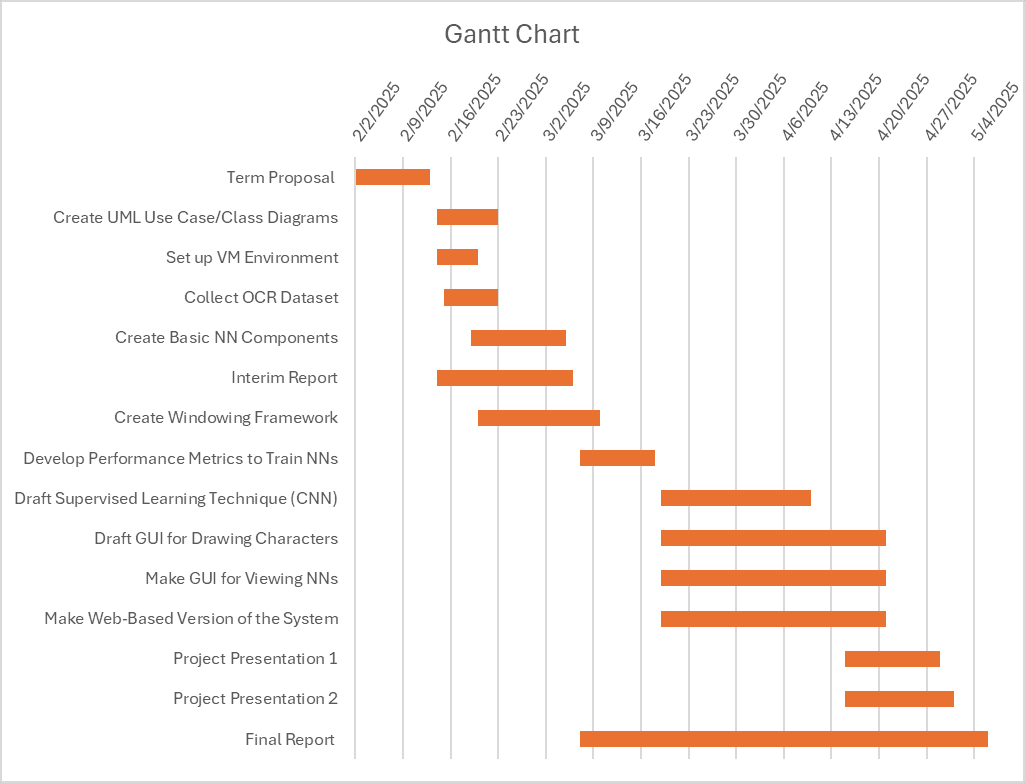
\includegraphics[width=15cm, height=10cm]{images/Colin's Gantt Chart.png}
\end{figure}
\subsection{Resource Table}
\begin{longtable}{|P{0.20\linewidth}|P{0.10\linewidth}|P{0.2\linewidth}|P{0.5cm}|}
  \caption{Resource Table} \\
  \hline
  \multicolumn{1}{|c|}{\textbf{Task}} & 
  \multicolumn{1}{|c|}{\textbf{People}} & 
  \multicolumn{1}{|c|}{\textbf{Hardware and Software}} &
  \multicolumn{1}{|c|}{\textbf{Special}}
  \\ [0.5ex]
  \hline
  \endfirsthead
  \hline
  \multicolumn{4}{|c|}{\textit{Continued from previous page}} \\ 
  \hline
  \textbf{Task} & \textbf{People} & \textbf{Hardware and Software} & \textbf{Special}\\ 
  \hline
  \endhead
  \hline
  \multicolumn{4}{|c|}{\textit{Continued on the next page}} \\ 
  \hline
  \endfoot
  \endlastfoot

  Term Proposal & Group & Latex and Excel & None\\
  \hline

  Create UML Use Case/Class Diagrams & Group & \textit{Dia} and \textit{draw.io} & None\\
  \hline

  Set Up VM Environment  & John Runyon & Computer and VM & None\\
  \hline

  Collect OCR Dataset & Colin and John & Computer and VM & None\\
  \hline

  Create Basic NN Components & Cole Johnson & \textit{openJDK22} and \textit{Java Language} & None \\
  \hline

  Interim Report & Group & \textit{LaTex} & None \\
  \hline

  Create Windowing Framework & Lauren & \textit{openJDK22} and \textit{Java Language} & None\\
  \hline

  Develop Performance Metrics to Train NNs & Cole and John & \textit{openJDK22} and \textit{Java Language} & None\\
  \hline

  Draft Supervised Learning Technique (CNN) & Group & Computer and VM & None\\
  \hline

  Draft GUI for Drawing Characters & Lauren & \textit{openJDK22} and \textit{Java Language}  & None\\
  \hline

  Make GUI for Viewing NNs & Cole and Lauren & \textit{openJDK22} and \textit{Java Language}  & None\\
  \hline

  Make Web-Based Version of the System & John & \textit{nginx}, \textit{JSweet}, and \textit{React} & None\\
  \hline

  Project Presentation & Group & \textit{Google Slides} and \textit{LaTex} & None \\
  \hline

  Final Report & Group & Latex & None \\
  \hline
\end{longtable}
\section{Project Resources}

\subsection{People}
\begin{enumerate}
  \item Colin Grandjean 
  \item Lauren Giles   
  \item Cole Johnson (Team Leader)
  \item John Runyon    
\end{enumerate}
\subsection{Hardware and Software Resources}
We plan to create our project using Java, version 22. 
To help automate our build and deployment processes, we are using Gradle. 
In order to facilitate version control, we use GitHub with Jira to keep track of our 
development process and task management. Each team member uses different 
code editors, depending on their preferences. We will be using primarily Latex to
write our reports and keep track of documentation.

\subsection{Special Resources}
The only possible special resource we may need for the project is a Virtual Machine 
to manage the development environment. Later, we will use
special software to try and port our java application to web, which may need
special considerations.
\section{Appendices}  

\subsection{Tasks Completed by Group Members}

\textbf{Cole:}
Drafted section 1 and section 2 of the proposal, and wrote some entires of the risk table.
Organized meetings and maintained a git repository for work on the final project. 
Brainstormed ideas and organized a task list along with all the other members
of the project.

\textbf{Colin:} 
Created task list, Gantt Chart, and Resource table. 
Transferred all of the information from the rough draft of our task list, which included tasks, 
dates, and people who are working on the tasks, into the project proposal. 
Completed all of section 3 except for the Hardware and Software section of the resource table.

\textbf{John:} 
Assisted in overall document formatting, 
including extended tables, alphabetical organization, 
and the risk table. Reviewed and improved grammar 
throughout the document. Contributed to meeting planning and organization to 
enhance workflow, streamline ideas and scope, and suggested process management 
strategies and software for project completion.

\textbf{Lauren:} 
Created the Jira project for tracking issues and overall development 
process using an Agile workflow as well as configuring the project to prepare for 
the start of the development process. Added information for the Project requirements 
section and aided in some of the planning of needed tasks during team meetings.
\end{document}
